\documentclass[14pt]{extarticle} 
\usepackage{amsmath,mathtools,amsfonts,amsthm,amssymb,hyperref}
\usepackage{wasysym,geometry,bussproofs,latexsym,parskip,bookmark}
\usepackage{mathtools,float,xcolor}
\newtheorem{defn}{Definition}
\newtheorem{thm}{Theorem}
\newtheorem{claim}{Claim}
\newtheorem{lemma}{Lemma}
\newcommand{\lbr}{\textcolor{red}{{\bf [\,}}}
\newcommand{\rbr}{\textcolor{blue}{{\bf ]\,}}}
\hypersetup{colorlinks,allcolors=blue,linktoc=all}
\geometry{a4paper} 
\geometry{margin=0.5in}
\title{Math for CS 2015/2019 solutions to ``In-Class Problems Week 5, Mon. (Session 10)''}
\author{https://github.com/spamegg1}
\begin{document}
\maketitle
\tableofcontents

\section{Problem 1}
The Elementary 18.01 Functions (F18’s) are the set of functions of one real variable defined recursively as follows:

{\bf Base cases:}

1. The identity function, $id(x) \Coloneqq x$ is an F18,

2. any constant function is an F18,

3. the sine function is an F18,

{\bf Constructor cases:}

If $f, g$ are F18’s, then so are

1. $f + g$, $fg$, $2^g$,

2. the inverse function $f^{-1}$,

3. the composition $f \circ g$.

\subsection{(a)}
(a) Prove that the function $1/x$ is an F18.

Warning: Don’t confuse $1/x = x^{-1}$ with the inverse $id^{-1}$ of the identity function $id(x)$. The inverse $id^{-1}$ is equal to $id$.
\begin{proof}
1. The identity function $id(x) = x$ is an F18.

2. So $2^id = 2^x$ is an F18 (by the 1st Constructor case).

3. $\log_2(x)$ is the inverse of $2^x$, so $\log_2(x)$ is an F18 (by the 2nd Constructor case).

4. The constant function $-1$ is an F18 (by the 2nd Base case).

5. By (3) and (4) $-\log_2(x)$ is an F18 (by the 1st Constructor case).

6. By (5), $2^{-\log_2(x)} = (2^{\log_2(x)})^{-1} = x^{-1} = 1/x$ is an F18 (by the 1st Constructor case).

(There is a little problem here: since $\log_2(x)$ is not real valued for $x \leq 0$, the function $f(x) \Coloneqq x^{-1}$ constructed this way is only defined for $x > 0$. To get an F18 equal to $1/x$ for all $x \neq 0$, use $(x / |x|) \cdot f(|x|)$, where $|x| = \sqrt{x^2}$.)
\end{proof}

\subsection{(b)}
(b) Prove by Structural Induction on this definition that the Elementary 18.01 Functions are closed under taking derivatives. That is, show that if $f(x)$ is an F18, then so is $f' \Coloneqq df/dx$. (Just work out 2 or 3 of the most interesting constructor cases; you may skip the less interesting ones.)
\begin{proof}
By Structural Induction on the definition of F18. The induction hypothesis is the above statement to be shown.

{\bf Base Cases.} We want to show that the derivatives of all the base case functions are in F18.

This is easy: for example, $\frac{d(id(x))}{dx} = 1$ is a constant function, and so is in F18. Similarly, $\frac{d(\sin(x))}{dx} = \cos(x)$ which is also in F18 since $\cos(x) = \sin(x + \pi/2)$ is in F18 by rules for constant functions, the identity function, sum, and composition with sine.

This proves that the induction hypothesis holds in the Base cases.

{\bf Constructor Case $f^{-1}$} Assume $f$ and $df/dx$ are in F18 to prove $\frac{df^{-1}(x)}{dx}$ is in F18. 

Letting $y = f(x)$, so $x = f^{-1}(y)$, we know from Leibniz’s rule in calculus that 
$$
\frac{df^{-1}(y)}{dy} = \frac{dx}{dy} = \frac{1}{\frac{dy}{dx}} \,\,\,\,\,\,\,\,(1)
$$

For example, 

$$
\frac{d\sin^{-1}(y)}{dy} = \frac{1}{\frac{d \sin(x)}{dx}} = \frac{1}{\cos(x)} = \frac{1}{\cos(\sin^{-1}(y))}
$$

Stated as in (1), this rule is easy to remember, but can easily be misleading because of the variable switching between x and y. It’s more clearly stated using variable-free notation:
$$
(f^{-1})' = (1/f') \circ f^{-1} \,\,\,\,\,\,\,\,(2)
$$

Now, since $f'$ is in F18 (by assumption), so are $1/f'$ (by part (a)) and $f^{-1}$ (by constructor rule 2.), and therefore so is their composition (by rule 3). Hence the righthand side of equation (2) defines a function in F18.

{\bf Constructor Case: $f \circ g$}. Assume $f, g, df/dx, dg/dx$ are in F18, to prove $d(f \circ g)(x)/dx$ is in F18.

The Chain Rule states that
$$
\frac{d(f(g(x)))}{dx} = \frac{df(g)}{dg}\cdot\frac{dg}{dx}
$$

Stated more clearly in variable-free notation, this is
$$
(f \circ g)' = (f' \circ g) \cdot g'
$$

The righthand side of this equation defines a function in F18 by constructor rules 3 and 1.

The other Constructor cases are similar, so we conclude that the induction hypothesis holds in all Constructor cases.

This completes the proof by structural induction that the statement holds for all $f$ in F18.
\end{proof}

\section{Problem 2}
Let $p$ be the string \lbr\rbr. A string of brackets is said to be erasable iff it can be reduced to the empty string by repeatedly erasing occurrences of $p$ (read from left-to-right, whenever you encounter an occurrence of $p$, erase it, keep moving right, when you reach the end, go back to the beginning, repeat). For example, here’s how to erase the string \lbr\lbr\lbr\rbr\rbr\lbr\rbr\rbr\lbr\rbr:

\begin{center}
\lbr\lbr\lbr\rbr\rbr\lbr\rbr\rbr\lbr\rbr $\to$ \lbr\lbr\rbr\rbr $\to$ \lbr\rbr $\to\lambda$
\end{center}

On the other hand the string \lbr\rbr\rbr\lbr\lbr\lbr\lbr\lbr\rbr\rbr is not erasable because when we try to erase, we get stuck:

\begin{center}
\lbr\rbr\rbr\lbr\lbr\lbr\lbr\lbr\rbr\rbr $\to$ \rbr\lbr\lbr\lbr\lbr\rbr $\to$ \rbr\lbr\lbr\lbr $\not\to$
\end{center}

Let Erasable be the set of erasable strings of brackets. Let RecMatch be the recursive data type of strings of matched brackets defined recursively:

{\bf Base case:} $\lambda \in$ RecMatch.

{\bf Constructor case:} If $s, t \in$ RecMatch, then \lbr$s$ \rbr$t \in$ RecMatch.

\subsection{(a)}
Use structural induction to prove that RecMatch $\subseteq$ Erasable.
\begin{proof}
We prove by structural induction on the definition of RecMatch that the predicate 
$$
P(x) \Coloneqq x \in \text{Erasable}
$$
is true for all $x \in$ RecMatch.

{\bf Base case:} $(x = \lambda)$ The empty string is erasable by definition of Erasable – it can be reduced to itself by erasing the substring $p =$\lbr\rbr exactly 0 times.

{\bf Constructor case:} ($x = $ \lbr $s$ \rbr $t$ for $s, t \in$ RecMatch). 

By structural induction hypothesis, we may assume that $s, t \in$ Erasable. So to erase $x$, erase $s$ and then erase $t$ to be left with the substring $p =$\lbr\rbr, and one more erasure leads to the empty string.

This completes the proof by structural induction, so we conclude that 
$$
\forall x(x \in \text{RecMatch} \text{ IMPLIES } x \in \text{Erasable})
$$
which by definition means that RecMatch $\subseteq$ Erasable.
\end{proof}

\subsection{(b)}
Supply the missing parts (labeled by “(*)”) of the following proof that Erasable $\subseteq$ RecMatch.
\begin{proof}
We prove by strong induction that every length $n$ string in Erasable is also in RecMatch. ($|x|$ denotes the length of string $x$.) The induction hypothesis is
$$
P(n) \Coloneqq \forall x((x \in \text{Erasable AND } |x| = n) \text{ IMPLIES } x \in \text{RecMatch})
$$

{\bf Base case:}
(*) What is the base case? Prove that $P$ is true in this case.

{\bf Solution.} The base case is $n = 0$. Now $P (0)$ is true because the empty string is the only string of length 0, and it is in RecMatch by the base case of the definition of RecMatch.

{\bf Inductive step:} To prove $P(n + 1)$, suppose $|x| = n + 1$ and $x \in$ Erasable. We need to show that $x \in$ RecMatch.

Let’s say that a string $y$ is an erase of a string $z$ iff $y$ is the result of erasing a single occurrence of $p$ in $z$.

Since $x \in$ Erasable and has positive length, there must be an erase, $y \in$ Erasable, of $x$. So $|y| = n$ and since $y \in$ Erasable, we may assume by induction hypothesis that $y \in$ RecMatch.

Now we argue by cases:

{\bf Case} ($y$ is the empty string):
(*) Prove that $x \in$ RecMatch in this case.

{\bf Solution.} In this case $x = p \in$ RecMatch.

{\bf Case} $y =$ \lbr $s$ \rbr $t$ for some strings $s, t \in$ RecMatch: Now we argue by subcases.

{\bf Subcase} $x = py$.

(*) Prove that $x \in$ RecMatch in this subcase.

{\bf Solution.} Let $t' \Coloneqq$ \lbr $s$ \rbr $t$ and $s'$ be the empty string. Then $x =$ \lbr $s'$ \rbr $t'$. But we know
$s', t' \in$ RecMatch, which implies that $x \in$ RecMatch because it is the result the RecMatch constructor step applied to $s', t'$.

{\bf Subcase} $x$ is of the form \lbr $s'$ \rbr $t$ where $s$ is an erase of $s'$:

Since $s \in$ RecMatch, it is erasable by part (b), which implies that $s' \in$ Erasable. But $|s'| < |x|$, so by induction hypothesis, we may assume that $s' \in$ RecMatch. This shows that $x$ is the result of the constructor step of RecMatch, and therefore $x \in$ RecMatch.

{\bf Subcase} $x$ is of the form \lbr $s$ \rbr $t'$ where $t$ is an erase of $t'$:

(*) Prove that $x \in$ RecMatch in this subcase.

{\bf Solution.} The proof is essentially identical to the previous case, with $t, t'$ in place of $s, s'$ :

Now $t$ is erasable by part (b), so $t' \in$ Erasable. But $|t'| < |x|$, so by induction hypothesis, we may assume that $t' \in$ RecMatch. This proves that $x$ is the result of the constructor
step of RecMatch and therefore $x \in$ RecMatch.

(*) Explain why the above cases are sufficient.

{\bf Solution.} The proofs of the remaining Subcases are just like this last one. Here is a list of these remaining subcases:

{\bf Case} $x =$ \lbr $ps$ \rbr $t$ (for some strings $s, t$)

{\bf Case} $x =$ \lbr $sp$ \rbr $t$ (for some strings $s, t$)

{\bf Case} $x =$ \lbr $s$ \rbr $pt$ (for some strings $s, t$)

{\bf Case} $x =$ \lbr $s$ \rbr $tp$ (for some strings $s, t$)

This completes the proof by strong induction on $n$, so we conclude that $P(n)$ holds for all $n \in \mathbb{N}$. Therefore $x \in$ RecMatch for every string $x \in$ Erasable. That is, Erasable $\subseteq$ RecMatch. 

Combined with part (a), we conclude that Erasable = RecMatch.
\end{proof}

\section{Problem 3}
Here is a simple recursive definition of the set, $E$, of even integers:


{\bf Definition.} Base case: $0 \in E$.

{\bf Constructor cases:} If $n \in E$, then so are $n + 2$ and $-n$.

Provide similar simple recursive definitions of the following sets:
\subsection{(a)}
The set $S \Coloneqq \{2^k 3^m 5^n \,\,|\,\, k, m, n \in \mathbb{N} \}$.
\begin{proof}
We can define the set $S$ recursively as follows:

$1 \in S$.

If $n \in S$, then $2n, 3n$, and $5n$ are in $S$.
\end{proof}

\subsection{(b)}
The set $T \Coloneqq \{2^k 3^{2k+m} 5^{m+n} \,\,|\,\, k, m, n \in \mathbb{N} \}$.
\begin{proof}
We can define the set $T$ recursively as follows:

$1 \in T$.

If $n \in T$, then $18n, 15n$, and $5n$ are in $S$.
\end{proof}

\subsection{(c)}
The set $L \Coloneqq \{(a,b) \in \mathbb{Z}^2 \,\,|\,\, a-b \text{ is a multiple of 3}\}$.
\begin{proof}
We can define the set $L$ recursively as follows:

$(0,0), (1,1), (2,2) \in L$.

If $(a,b) \in L$, then $(a-3,b), (a+3,b), (a,b+3)$, and $(a,b-3)$ are in $L$.
\end{proof}

Let $L'$ be the set defined by the recursive definition you gave for $L$ in the previous part. Now if you did it right, then $L' = L$, but maybe you made a mistake. So let’s check that you got the definition right.

\subsection{(d)}
Prove by structural induction on your definition of $L'$ that $L' \subseteq L$.
\begin{proof}
For the $L'$ defined above, a straightforward structural induction shows that if $(c, d) \in L'$, then $(c, d) \in L$. 

Namely, each of the base cases in the definition of $L'$ are in $L$ since $3 \mid 0$. 

For the constructor cases, we may assume $(a, b) \in L$, that is $3 \mid (a - b)$, and must prove that $(a \pm 3, b) \in L$ and $(a, b \pm 3) \in L$. 

In the first the case, we must show that $3 \mid ((a \pm 3) - b)$. But this follows immediately because $((a \pm 3) - b) = (a - b) \pm 3$ and 3 divides both $(a - b)$ and 3. 

The other constructor case $(a, b \pm 3)$ follows in exactly the same way. So we conclude by structural induction on the definition of $L'$ that $L' \subseteq L$.
\end{proof}

\subsection{(e)}
Confirm that you got the definition right by proving that $L \subseteq L'$.
\begin{proof}
Conversely, we must show that $L \subseteq L'$. 

So suppose $(c, d) \in L$, that is, $3 \mid (c - d)$. This means that $c = r + 3k$ and $d = r + 3j$ for some $r \in \{0, 1, 2\}$ and $j, k \in \mathbb{Z}$. 

Then starting from base case $(r, r) \in L'$, we can apply the $(a \pm 3, b)$ constructor rule $|k|$ times to conclude that $(c, r) \in L'$, and then apply the $(a, b \pm 3)$ rule $|j|$ times to conclude that $(c, d) \in L'$. 

This implies that $L \subseteq L'$, which completes the proof that $L = L'$.
\end{proof}

\subsection{(f)}
See if you can give an unambiguous recursive definition of $L$.
\begin{proof}
This is tricky. Here is an attempt:

{\bf Base cases: }

$(0, 0), (1, 1), (2, 2), (-1, -1), (-2, -2), (-3, -3)(1, -2), (2, -1), (-1, 2), (-2, 1) \in L$.

Now the idea is to constrain the constructors so the two coordinates have absolute values that increase differing by at most 1, then one coordinate only can continue to grow in absolute value.

Let
$$
Sg(x) = \left\{
     \begin{array}{lr}
       1 & \text{if } x \geq 0 \\
       -1 & \text{if } x < 0 \\
     \end{array}
   \right.
$$

Constructors: If $(a, b) \in L$, then:

if $||a| - |b|| \leq 1$, then $(a + 3\cdot Sg(a), b + 3 \cdot Sg(b)), (a + 3\cdot Sg(a), b), (a, b + 3\cdot Sg(b)) \in L$,

if $|a| > |b| + 1$, then $(a + 3\cdot Sg(a), b) \in L$,

if $|b| > |a| + 1$, then $(a, b + 3\cdot Sg(b)) \in L$.
\end{proof}

\section{Problem 4}
{\bf Definition.} The recursive data type, binary-2PTG, of binary trees with leaf labels, $L$, is defined recursively as follows:

{\bf Base case:} $\langle leaf, l\rangle \in$ binary-2PTG, for all labels $l \in L$.

{\bf Constructor case:} If $G_1, G_2 \in$ binary-2PTG, then
$$
\langle bintree, G_1, G_2\rangle \in \text{binary-2PTG.}
$$

The size, $|G|$, of $G \in$ binary-2PTG is defined recursively on this definition by:

{\bf Base case:} $| \langle leaf, l \rangle| \Coloneqq 1$ for all $l \in L$.

{\bf Constructor case:} $|\langle bintree, G_1, G_2\rangle| \Coloneqq |G_1| + |G_2| + 1$.

For example, the size of the binary-2PTG, $G$, pictured below, is 7.
\begin{figure}[ht!]
\centering
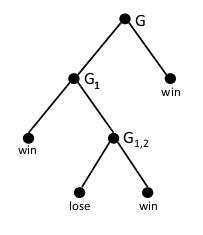
\includegraphics[scale=1.0]{bintree.png}
\end{figure}

\subsection{(a)}
Write out (using angle brackets and labels $bintree$, $leaf$, etc.) the binary-2PTG, $G$, pictured above.
\begin{proof}
At the bottom we have two leaves: $\langle leaf, lose\rangle$ and $\langle leaf, win\rangle$.

These are connected to $G_{1,2} \Coloneqq \langle bintree, \langle leaf, lose\rangle, \langle leaf, win\rangle \rangle$.

This is connected to $G_{1}$ with a leaf on the left: 
$$
G_1 \Coloneqq \langle bintree, \langle leaf, win\rangle, \langle bintree, \langle leaf, lose\rangle, \langle leaf, win\rangle \rangle\rangle
$$
Finally we add another leaf on the right to get $G$:
$$
G \Coloneqq \langle bintree, \langle bintree, \langle leaf, win\rangle, \langle bintree, \langle leaf, lose\rangle, \langle leaf, win\rangle \rangle\rangle, \langle leaf, win\rangle\rangle
$$
\end{proof}

The value of flatten$(G)$ for $G \in$ binary-2PTG is the sequence of labels in $L$ of the leaves of $G$. For example, for the binary-2PTG, $G$, pictured above, 

\begin{center}
flatten$(G)$ = (win, lose, win, win)
\end{center}

\subsection{(b)}
(b) Give a recursive definition of flatten. (You may use the operation of concatenation (append) of two sequences.)
\begin{proof}
{\bf Base Case.} flatten$(\langle leaf, l\rangle) \Coloneqq (l)$ for all labels $l \in L$.

{\bf Constructor Case.} flatten$(\langle bintree, G_1, G_2\rangle) \Coloneqq$ flatten$(G_1)$ concat flatten$(G_2)$ for all $G_1, G_2 \in$ binary-2PTG.
\end{proof}

\subsection{(c)}
(c) Prove by structural induction on the definitions of flatten and size that 
$$
2 \cdot \text{length}(\text{flatten}(G)) = |G| + 1
$$
\begin{proof}
{\bf Base Case.} In this case $G = \langle leaf, l\rangle$. So $|G| = 1$.

$2 \cdot$length(flatten$(\langle leaf, l\rangle)$) = $2 \cdot$length($(l)$) = $2 \cdot 1 = 2 = 1+1 = |G| + 1$.

{\bf Constructor Case.} In this case $G = \langle bintree, G_1, G_2\rangle$. Note that by the constructor case of the definition of size, we have $|G| = |G_1| + |G_2| + 1$.

Assume $G_1, G_2 \in$ binary-2PTG and assume:
$$
2 \cdot \text{length}(\text{flatten}(G_1)) = |G_1| + 1
$$
$$
2 \cdot \text{length}(\text{flatten}(G_2)) = |G_2| + 1
$$
Notice that for two sequences seq1, seq2, we have 
\begin{center}
length(seq1 concat seq2) = length(seq1) + length(seq2).
\end{center}
Then:
$$
\begin{array}{lcl}
2 \cdot \text{length}(\text{flatten}(G)) & = & 2 \cdot \text{length}(\text{flatten}(G_1) \text{ concat } \text{flatten}(G_1)) \\
 & = & 2 \cdot (\text{length}(\text{flatten}(G_1)) + \text{length}( \text{flatten}(G_1))) \\
& = & 2 \cdot (\frac{|G_1| + 1}{2} + \frac{|G_2| + 1}{2}) \\
& = & |G_1| + 1 + |G_2| + 1 \\
& = & (|G_1| + |G_2| + 1) + 1\\
& = & |G| + 1.
\end{array}
$$
\end{proof}

\end{document}
